%lesson 3 of 09/03/2026
\item $\mathbf{0\leq E\leq V_0}$
   Classicamente le zone $I$ e $III$ sono proibite, ma, come è noto, non lo sono quantisticamente:
   l'equazione differenziale diventa
   $$
   \begin{dcases}
       \psi'' - \beta^2\psi = 0 & |x| >a\\
       \psi'' + k^2\psi = 0 & |x| <a
   \end{dcases}
   $$
   con $\beta^2 = \frac{-2mE}{\hbar^2}>0$ e $k^2=\frac{2m(E-V_0)}{\hbar^2}>0$.

   Come è noto, le soluzioni in $|x|>a$ sono del tipo $\psi(x) = Ae^{\beta x}+Be^{-\beta x}$ e, per
   garantire che $\psi(x)$ sia almeno una distribuzione regolare, bisogna annullare i termini che divergono,
   cioè l'esponenziale positivo (negativo) per $x>0$ ($x<0$).
   La soluzione è dunque

   $$
    \psi(x) =
    \begin{dcases}
	Ae^{\beta x} & x< -a \\
	Ce^{ikx}+De^{-ikx} & -a<x<a \\
	Ge^{-\beta x} & x>a
    \end{dcases}
   $$
Che può essere riscritta in termini di funzioni pari o dispari, come specificato prima:
$$
\psi_P(x) =
    \begin{dcases}
	Ae^{\beta x} \\
	B\cos(kx) \\
	Ae^{-\beta x}
    \end{dcases}
    \quad
\psi_D(x) = 
    \begin{dcases}
	Ce^{\beta x} &x< -a\\
	D\sin(kx) &-a<x<a\\
	-Ce^{-\beta x}&x>a
    \end{dcases}
$$
Le condizioni di continuità di $\psi(x)$ e $\psi'(x)$ sono due sistemi lineari a due equazioni e due
incognite: se il sistema non è singolare ($\det M_{\text{coeff}} \neq 0$), l'unica soluzione è $\psi(x)\equiv 0$,
soluzione non ammissibile, mentre se è singolare le condizioni sui determinanti sono, rispettivamente per
$\psi_P$ e $\psi_D$, $k\tan(ka)=\beta$ e $k\cot(ka)=\beta$.

Queste condizioni sono facilmente risolubili numericamente definendo le quantità
\begin{align*}
    \xi &= ka\\
    \eta &= \beta a\\
    r^2 &= \frac{-2m}{\hbar^2}V_0 = \xi^2+\eta^2
\end{align*}
e diventano
$$
\begin{dcases}
\xi\tan(\eta) = \eta\\
\xi^2 + \eta^2 = r^2
\end{dcases}
\quad
\begin{dcases}
\xi\cot(\eta) = \eta\\
\xi^2 + \eta^2 = r^2
\end{dcases}
$$

Nelle figure 3.1 e 3.2 sono rappresentate le soluzioni dei sistemi.

\begin{multicols}{2}

\begin{figure}[H]
    \centering
    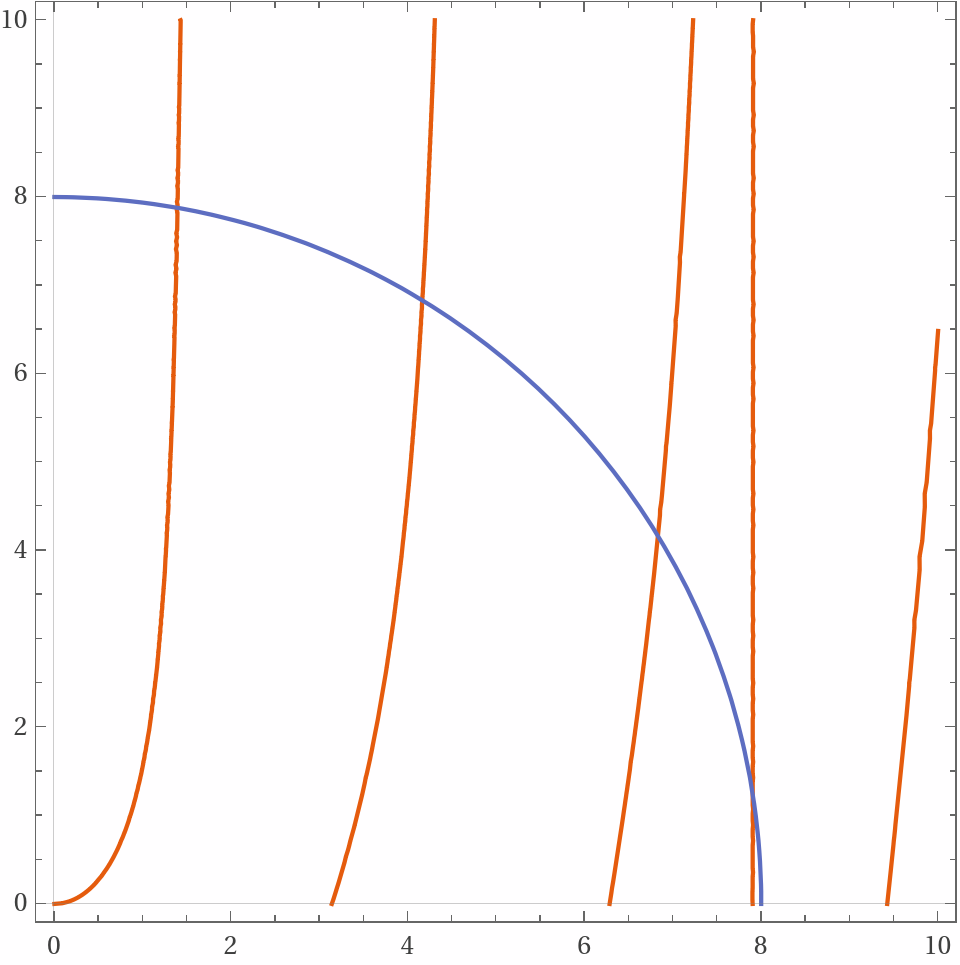
\includegraphics[width = \linewidth]{./even_well.png}
    \caption{\small{Soluzioni per le autofunzioni pari}}
\end{figure}
\begin{figure}[H]
    \centering
    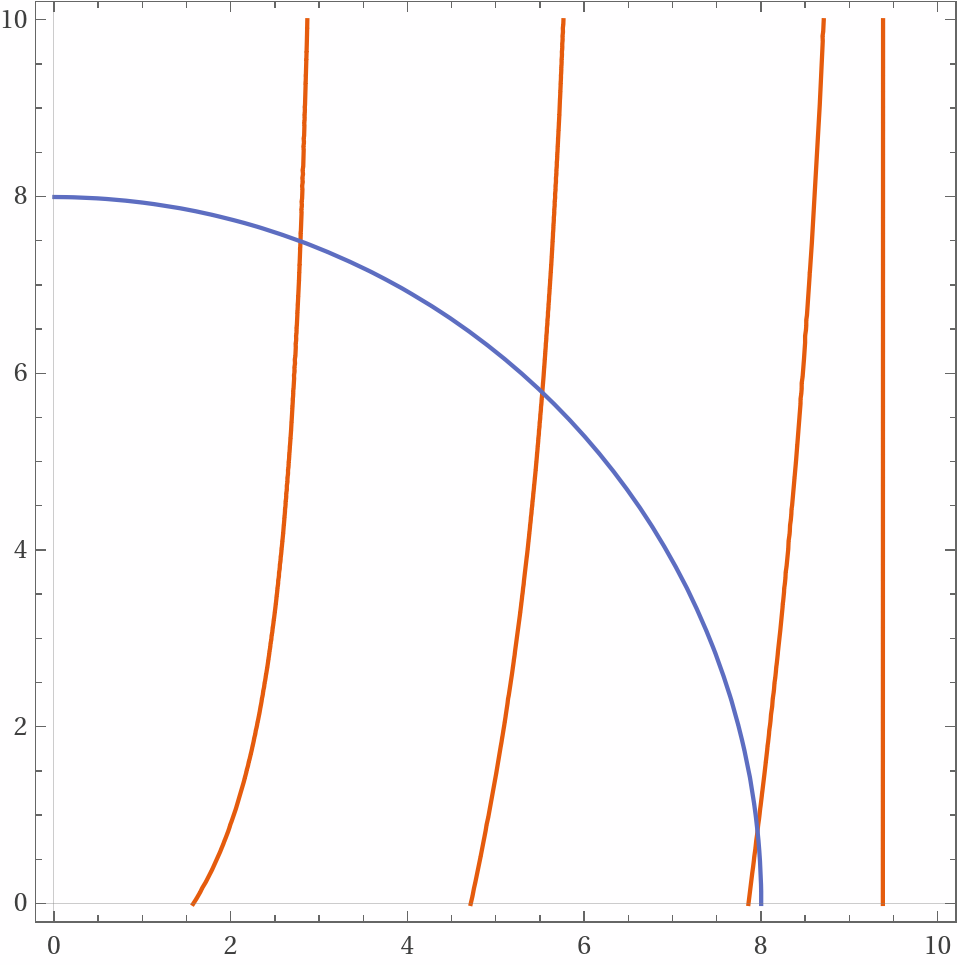
\includegraphics[width = \linewidth]{./odd_well.png}
    \caption{\small{Soluzioni per le autofunzioni dispari}}
\end{figure}
\end{multicols}

Questi sistemi hanno un insieme discreto e finito di soluzioni e questo quantizza l'energia.

\textbf{Oss.} Come si nota dalla figura 3.1, lo stato fondamentale è pari ed è l'unico che esiste per ogni
valore di $r$, cioè di $V_0$. Queste caratteristiche sono generali, come si vedrà in seguito.
\newpage
\item $\mathbf{E<V_0}$
Classicamente questo caso è completamente proibito; quantisticamente la soluzione è fatta da soli
esponenziali reali

$$
 \psi(x) =
    \begin{dcases}
	Ae^{\beta_I x} & x< -a \\
	Be^{\beta_{II} x}+De^{-\beta_{II} x} & -a<x<a \\
	Ge^{-\beta_I x} & x>a
    \end{dcases}
$$
A differenza del caso precedente, il sistema imposto dalle condizioni di continuità non può mai essere
singolare, quindi questo caso \textbf{non è possibile} nemmeno nella meccanica quantistica.
\end{itemize}

Ricapitolando, l'hamiltoniana di una buca finita di potenziale ha sia spettro discreto $Spd\subset[V_0,0]$
sia spettro continuo $Spc = [0,\infty)$.

\subsubsection{Casi limite}
Si trattano ora tre casi limite del problema appena risolto.
\begin{itemize}[leftmargin=*]
\item \textbf{Buca infinita}

Per $V_0\to-\infty$, si ha solo spettro discreto ed esso diventa infinito:

la condizione $\xi^2+\eta^2 = \frac{-2m}{\hbar^2}V_0\to\infty$ e, in questo limite, le soluzioni dei sistemi
sono gli asintoti di $\tan(x)$ e $\cot(x)$, cioè $\xi = n\pi$, la relazione $\xi^2+\eta^2=r^2$ diventa

    $$n^2\pi^2 = a^2(k^2+\beta^2)=\frac{2ma^2}{\hbar^2}(E-V_0) \to E_n-V_0 = \frac{\pi^2\hbar^2}{2ma^2}$$
\item $\mathbf{V_0\to0}$

    In questo limite, $r^2\to 0$ ed esiste un unico stato legato pari, con $\xi\to0$ e $\eta\to 0$:

    $\eta = \xi\tan(\xi)\approx\xi^2$ e dunque $\eta^2+\eta = r^2 \to \eta\approx r^2$; ricordando le 
    definizioni di queste quantità si trova $E = \frac{-2ma^2}{\hbar^2}V_0^2$
\item $\mathbf{V(x)=-\delta(x)}$

    Per avere una delta di Dirac, non basta far tendere la profondità a $\infty$ e la larghezza a 0, ma
    serve che l'area sia costante: si definisce $V_0 =\frac{-A}{2a}$ e
    $\lim\limits_{a\to0}V(x) = -A\delta(x)$.

    $r^2 = \frac{-2m}{\hbar^2}a^2V_0^2=\frac{mA}{\hbar^2}a\to0$ per $a\to 0$: si possono utilizzare i limiti
    del caso precedente e trovare che c'è un solo stato legato con energia
    $E = \frac{-2ma^2}{\hbar^2}V_0^2 = \frac{-m}{2\hbar^2}A^2$

\end{itemize}


\subsection{Risultati generali sui potenziali}
\subsubsection{Potenziale attrattivo}
Si dice potenziale attrattivo un potenziale $V(\vec{x})$ tale che
$$\lim\limits_{|\vec{x}|\to\infty}V(\vec{x}) = 0,\quad V(\vec{x})<0$$
Per i potenziali di questo tipo valgono i seguenti risultati

\begin{itemize}
    \item $\mathbf{E<0} \to \psi\in L^2(\mathbb{R}^3)$, cioè 
	$\psi(\vec{x}) \underset{|\vec{x}|\to\infty}\sim e^{-\beta |\vec{x}|}$.
	
	Infatti l'equazione di Schrödinger
	$\frac{-\hbar^2}{2m}\laplacian\psi+V\psi=E\psi$ è asintoticamente equivalente
	a $\laplacian\psi - \beta^2\psi \sim 0$, che ha come soluzione proprio
	$\psi(\vec{x}) \underset{|\vec{x}|\to\infty}\sim e^{-\beta |\vec{x}|}$;
	essendo $\psi$ quadrato-sommabile, $E\in Spd(H)$
    
	Si ha inoltre che $\forall \epsilon>0, \exists V\subset\mathbb{R}^3$ t.c.
	$\int_{V}^{}d^3x|\psi|^2 = 1-\epsilon$, come conseguenza della
	quadrato-sommabilità di $\psi$.
    \item $\mathbf{E>0} \to \psi$ di particella libera.

	Infatti la soluzione asintotica dell'equazione di Schrödinger è
	$\psi(\vec{x})\underset{|\vec{x}|\to\infty}\sim
	\frac{1}{(2\pi)^{3/2}}e^{i\vec{k}\cdot\vec{x}}$, che non è normalizzabile,
	dunque $E\in Spc(H)$
\end{itemize}
\subsubsection{Potenziali limitati inferiormente}
Si consideri un'Hamiltoniana di un sistema di $N$ particelle 
$$H = \sum_{i=1}^{N}\frac{p_i^2}{2m_i}+ V(\vec{x_1},...,\vec{x_N})$$

\noindent\fbox{%
    \parbox{\textwidth}{%
   \textbf{Teorema}

Se il potenziale è limitato inferiormente, cioè $\exists V_0$ t.c
$V>V_0\;\forall \vec{x_i}\in\mathbb{R}^{3N}$, allora lo spettro energetico è
limitato inferiormente, $\exists E_{min}>V_0$.

\textbf{Dimostrazione, Spd(H)}

$\forall \ket{\psi}\in\mathcal{H},\;\bra{\psi}H\ket{\psi} =
\bra{\psi}T\ket{\psi}+\bra{\psi}V\ket{\psi}.$

Per $T$ vale: 
$$\bra{\psi}T\ket{\psi} =
\sum_{i=0}^{N}\frac{1}{2m_i}\bra{\psi}p_i^{\dagger}p_i\ket{\psi} = 
\sum_{i=0}^{N}\frac{1}{2m_i}||p_i\ket{\psi}||^2>0$$ 
Per $V$ vale:
$$\bra{\psi}V\ket{\psi} = \int_{}^{}dxdy \bra{\psi}\ket{x}\bra{x}V\ket{y}\bra{y}
\ket{\psi} = \int_{}^{}dx V(x)|\psi|^2 \geq V_0\bra{\psi}\ket{\psi} = V_0$$
dove si è indicato con $x,y$ l'insieme di tutte le $3N$ coordinate.

Si ha dunque che $\langle H \rangle > V_0$ \textbf{QED}

\textbf{Dimostrazione, Spc(H)}

Si consideri ora $\bra{\psi}(H-E)\ket{\psi}>V_0-E := C$ per il risultato precedente; 
per assurdo, si assuma $E<V_0 \to C>0$.

Allora $\bra{\psi}(H-E)\ket{\psi} = |\bra{\psi}(H-E)\ket{\psi}| \leq
||\ket{\psi}||\,||(H-E)\ket{\psi}||$ e si ha
$$
||\ket{\psi}||\,||(H-E)\ket{\psi}||>C \to \frac{||(H-E)\ket{\psi}||}{||\ket{\psi}||}>
\frac{C}{||\ket{\psi}||^2}=C>0
$$
Prendendo l'Inf di questa espressione si trova
$
\inf\limits_{\ket{\psi}\in\mathcal{H}} \frac{||(H-E)\ket{\psi}||}{||\ket{\psi}||}>
\bar{C}>0
$

Cioè la definizione di $E$ punto regolare per $H$, si ha dunque che se $E<V_0$,
allora $E\not\in Sp(H)$.

\textbf{QED}
    }%
}




